\hei{34题、结合材料回答问题:}

\qquad \kai{人类每天都在产生垃圾,垃圾总量一天比一天多,由此带来的问题非常棘手。不产生垃圾是不可能的。既然如此,那就退而求其次,倡导大家减少垃圾。然而,减到多少才是少?这里并没有一个标准。而且从总体上看,生产和消费必然产生垃圾,减少垃圾很可能抑制生产和消费。接着往后退,把垃圾收集起来填埋或者焚烧。但填埋只是把垃圾从地上转移到地下,既与人争地,也有再次污染土壤和水源的隐患。焚烧不过是把污染从地上移到空中,产生二恶英等有害物质。}

\qquad \kai{于是,人们进一步追问:还有没有比填埋、焚烧更好的出路?这时候,一句“垃圾是放错地方的资源”让人茅塞顿开,垃圾可以回收利用,乃再生资源。但变废为“宝”前提是垃圾的分类投放——别把垃圾放错了地方。何谓放错?到处乱扔是放错,收集时搅混在一起也是放错。不同的垃圾只有往不同的地方放,才能实现资源的价值。即使还免不了要填埋、焚烧那些没有利用价值的垃圾,也得把它们分出来。}

\qquad \kai{垃圾分类举手之劳换出绿色,好处多多不言而喻,但如何让人们乐而为之?2009年5月起,上海开始普遍推广新的垃圾分类概念,开展以“换出更绿色的上海”为名义的“绿色帐户”活动。何为绿色帐户?就是居民对垃圾进行分类回收,积分换取环保小礼品:再生纸笔记本、绿色小植物、环保手电筒……上海推出“绿色帐户”的实践说明,办法是可以想出来的,关键是愿不愿意琢磨。中国的垃圾问题不比哪个国家小,我们只能“没有退路就多想出路”。}

\begin{flushright}\kai{摘编自《人民日报》}\end{flushright}

(1) 从实践是人和自然关系的基础的角度说明为什么“垃圾是放错地方的资源”?(5分)

(2) 运用矛盾分析方法说明“没有退路就多想出路”。(5分)

\clearpage

\hei{35题、结合材料回答问题:}

\hei{材料1}

\qquad \kai{成思危,著名经济学家,原民建中央主席,九届、十届全国人大常委会副委员长。谈到我国政党制度,他深有体会地说:“西方的政党制度是‘打橄榄球’,一定要把对方压倒。我们的政党制度是‘唱大合唱’,民主党派和中国共产党的合作共事是为了一个共同的目标,为了保持社会的和谐。要大合唱,就要有指挥,这个指挥无论从历史还是现实来看,都只有中国共产党才能胜任。”海外有评论说中国的民主党派人士在政府任职多是“坐虚位”、“无实权”,成思危说,这不符合实际情况,中国的民主党派不是“政治花瓶”。“在担任化工部副部长的时候,我对自己负责范围内的工作是完全有权作出决策的。作为全国人大常会副委员长,我负责证券法、农村金融的执法检查。我和中共党籍的副委员长一样,也是独当一面的。”}

\hei{材料2}

\qquad \kai{第十一届全国人大一次会议以来,全国共有18.7万民主党派、无党派人士当选各级人大代表。其中,全国人大常委会副委员长6人,省级人大常委会副主任35人。2人分别担任国务院科技部、卫生部部长。2007年有18人担任最高人民法院、最高人民检察院和中央国家机关部委领导职务副职。}

\qquad \kai{20世纪90年代以来,中共中央加强同各民主党派的协商,内容不断充实,程序逐步规范。据统计,1990年至2009年6月,中共中央、国务院直接召开或委托有关部门召开的协商会、座谈会、情况通报会就有287次,其中,中共中央总书记主持召开或出席的就有85次。各民主党派中央、无党派代表人士向中共中央、国务院及有关方面提出建议260多项,各民主党派地方组织提出各项建议9万多项。如关于三峡工程、耕地保护、两岸“三通”、西部大开发、中部崛起、东北地区等老工业基地振兴、建设社会主义新农村、青藏铁路沿线发展、国家级综合配套改革实验区、实施可持续发展战略、制定和实施“十一五”规划等方面提出的建议,得到了中共中央、国务院的高度重视和采纳。}

\begin{flushright}\kai{材料1、材料2摘编自《光明日报》}\end{flushright}

(1) 从“打橄榄球”和“唱大合唱”的形象比较中,说明我国政党制度的特点和优点。(5分)

(2) 我国各民主党派在社会主义建设中如何发挥参政议政的作用?(5分)

\clearpage

\hei{36. 结合材料回答问题:}

\hei{材料1}

\qquad \kai{2011年是中国共产党成立90周年。在这90年里,党走过了不平凡的历程。}

\qquad \kai{中华人民共和国成立前夕,毛泽东在一篇文章中指出:“一九一七年的俄国革命唤醒了中国人,中国人学得了一样新的东西,这就是马克思列宁主义。中国产生了共产党,这是开天辟地的大事变。”}

\begin{flushright}\kai{摘自《毛泽东选集》}\end{flushright}

\hei{材料2}

\qquad \kai{最近,有一本名为《苦难辉煌》的党史专著,颇受广大读者欢迎。}

\qquad \kai{在这部著作中,作者一再追问:为什么中国共产党从最初的几十个人,仅仅经过20多年的发展,就打败了强大的对手,取得了辉煌的胜利,建立了新中国?历史给国民党很多机会,却只给共产党很少机会,但是共产党抓住了这仅有的机会,实现了中国革命的胜利。这又是为什么?}

\qquad \kai{中国共产党从几十人的小党发展到今天7000多万人的大党,中国人民解放军从南昌起义后剩下不到800人到今天的威武雄狮,党和军队为何由小到大,由弱到强,筚路蓝缕,披荆斩棘?中国共产党的力量来自哪里?中国人民解放军的力量来自哪里?}

\qquad \kai{作者回答:我们拥有一批顶天立地的真人。他们不为钱,不为官,不怕苦,不怕死,只为胸中的主义和心中的信仰。}

\begin{flushright}\kai{摘编自 《人民日报》、《光明日报》}\end{flushright}

(1) 为什么说中国共产党的成立“是开天辟地的大事变?(4分)

(2) 结合中国共产党成立以来中国社会变革的历程,说明“主义”和“信仰”是怎样成为“力量”的?(6分)

\clearpage

\hei{37. 结合材料回答问题:}

\qquad \kai{郭明义,鞍山钢铁集团矿山公司齐大山铁矿采场公路管理员。几十年来,他照着雷锋那样去做,“把雷锋的道路作为自己的人生选择,把雷锋的境界作为自己的人生追求”,连续15年每天提前2小时上班,相当于多奉献了5年的工作量;连续20年先后55次无偿献血、捐献血小板,累计近6万毫升;连续16年为希望工程、工友、灾区群众捐款12万元,资助180多名特困生。可是,他一家至今还是住在一间不过40平米的旧楼房里。}

\qquad \kai{有人曾不解地问郭明义,你这么做究竟值不值得?“如果发出一点光,放出一点热,能够换来孩子幸福的笑脸,换来他人生命之花的绽放,换来人与人之间的温暖和谐,这样的人生,我无怨无悔!”“给人温暖就是给自己幸福”。他是这样说的,也是这样做的。}

\qquad \kai{30年来,郭明义就像一支火把燃烧着自己,也燃旺着志愿者和社会上更多人的爱心。他8次发起捐献造血干细胞的倡议,得到1700多人的响应;他7次发起献血的建议,600多人无偿献出15万毫升热血;他发起成立遗体(器官)捐献志愿者俱乐部,汇聚了200多名志愿者;他发起成立“郭明义爱心联队”,从12人已经发展到2800多人,捐款40余万元、资助特困生1000多名。}

\qquad \kai{郭明义的精神是一块磁石,在鞍钢、在辽宁、在全国吸引汇集越来越多的人加入爱心行动,为他人奉献、为社会分忧、为国家尽责,凝聚成巨大的道德力量,推进着当代中国社会稳定和谐发展。郭明义的先进事迹体现了“简单中的伟大”。}

\begin{flushright}\kai{摘编自《人民日报》}\end{flushright}

(1) 如何理解“给人温暖就是给自己幸福”?(6分)

(2) 为什么说郭明义的先进事迹是“简单中的伟大”?(4分)

\clearpage

\hei{38题、结合材料回答问题:}

\qquad \kai{金融危机发生后,某些西方国家的政要、媒体经常发表关于中国的言论,有“独秀”或“救世”之说、也有“责任”之论……林林总总,用词翻新。人们可看到一白一红“两张脸”:唱红脸者夸大中国的经济表现,动辄将一切不符合实际的高帽加诸中国,仿佛中国真的是世界经济的救世主。唱白脸者却将国际金融危机,全球失衡等责任归到中国头上。无论是明“捧”实“压”,还是借“批”卸“责”,万变不离其宗的都是鼓噪“中国责任论”。这既暴露出他们所谓“中国责任”的用心,也反映出其对“真实中国”的误解。}

\begin{center}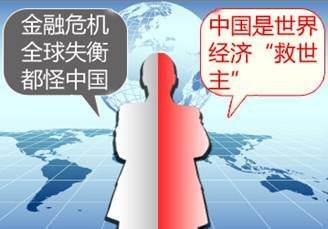
\includegraphics{2011.jpg}\end{center}

针对材料所反映的西方某些人士对中国的“捧”与“批”,谈谈什么是“真实的中国”以及中国的“责任”是什么。(10分)
